\documentclass{article}
\usepackage[utf8]{inputenc}
\usepackage{amsmath}
\usepackage{amsfonts}
\usepackage{amssymb}
\usepackage{tikz}

\begin{document}

\section*{Exercício 6 - Seção 15.6}
\textbf{Enunciado:} Calcular o volume da região que está acima do cone $z = \sqrt{x^2 + y^2}$ e abaixo da esfera $x^2 + y^2 + z^2 = 9$.

Primeiro, vamos traçar um esboço da região. A figura abaixo mostra a seção transversal da região. 

\begin{center}
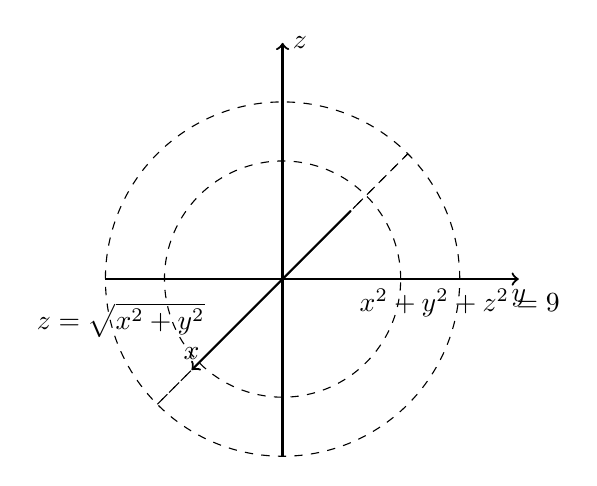
\begin{tikzpicture}[scale=1.5]
\draw[thick,->] (-1.5,0,0) -- (2,0,0) node[below]{$y$};
\draw[thick,->] (0,-1.5,0) -- (0,2,0) node[right]{$z$};
\draw[thick,->] (0,0,-1.5) -- (0,0,2) node[above]{$x$};
\draw[dashed] (0,0,0) circle[radius=1];
\draw[dashed] (0,0,0) -- (1,1,1);
\draw[dashed] (0,0,1) -- (1,1,1);
\draw[dashed] (0,0,0) circle[radius=1.5];
\draw[dashed] (0,0,0) -- (0,0,1.5);
\draw[dashed] (0,0,1.5) -- (-1.06,-1.06,0);
\draw[dashed] (0,0,1.5) -- (1.06,1.06,0);
\draw[dashed] (-1.06,-1.06,0) -- (1.06,1.06,0);
\node[above left] at (0,0,1.5) {$z=\sqrt{x^2+y^2}$};
\node[below] at (1.5,0,0) {$x^2+y^2+z^2=9$};
\end{tikzpicture}
\end{center}

Para calcular o volume da região, usaremos uma integral tripla. Como a região é simétrica em relação ao eixo $z$, podemos usar coordenadas cilíndricas. As equações de transformação são:

\begin{align*}
x &= r\cos\theta \\
y &= r\sin\theta \\
z &= z
\end{align*}

O cone $z = \sqrt{x^2 + y^2}$ pode ser escrito em coordenadas cilíndricas como $z = r$. A esfera $x^2 + y^2 + z^2 = 9$ pode ser escrita como $r^2 + z^2 = 9$. Como a região está abaixo da esfera, temos $z \leq \sqrt{9-r^2}$. Portanto, a integral tripla é:

\begin{equation*}
V = \iiint_D dV = \int_0^{2\pi} \int_0^3 \int_0^r r dz dr d\theta
\end{equation*}

A região de integração $D$ é o conjunto de pontos $(r, \theta, z)$ que satisfazem as desigualdades acima. A integral interna em $z$ varia de 0 a $r$, a integral do meio em $r$ varia de 0 a 3, e a integral externa em $\theta$ varia de 0 a $2\pi$.

Resolvendo as integrais, obtemos:

\begin{align*}
V &= \int_0^{2\pi} \int_0^3 \int_0^r r dz dr d\theta \\
&= \int_0^{2\pi} \int_0^3 \frac{1}{2}r^2 dr d\theta \\
&= \int_0^{2\pi} \frac{1}{2} \left[ \frac{1}{3}r^3 \right]_0^3 d\theta \\
&= \frac{9}{2}\pi
\end{align*}

Portanto, o volume da região é $\frac{9}{2}\pi$.

\newpage

\section*{Exercício 10 - Seção 15.6}
\textbf{Enunciado:} A região $E$ é definida pela desigualdade $x^2 + y^2 \leq z^2$ e $z^2 \leq 1$. Calcule

$$\iiint_E z^2 dV$$

\textbf{Resolução:}

Para resolver a integral tripla, primeiro precisamos determinar os limites de integração. A região $E$ é definida por $x^2 + y^2 \leq z^2$ e $z^2 \leq 1$, ou seja, é a região entre um cone circular e uma esfera unitária. A figura a seguir ilustra a região $E$:

\begin{center}
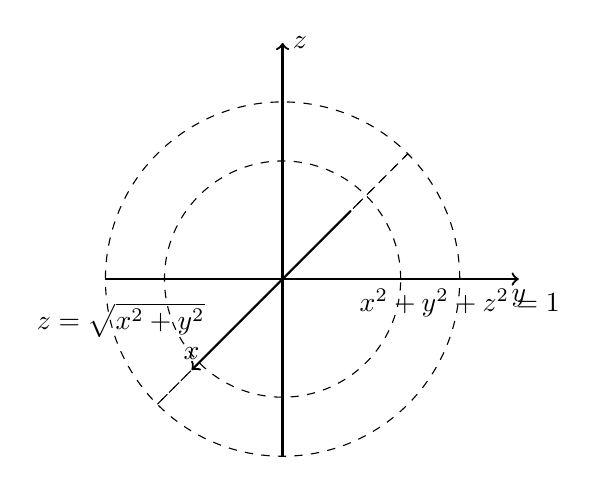
\begin{tikzpicture}[scale=1.5]
\draw[thick,->] (-1.5,0,0) -- (2,0,0) node[below]{$y$};
\draw[thick,->] (0,-1.5,0) -- (0,2,0) node[right]{$z$};
\draw[thick,->] (0,0,-1.5) -- (0,0,2) node[above]{$x$};
\draw[dashed] (0,0,0) circle[radius=1];
\draw[dashed] (0,0,0) -- (1,1,1);
\draw[dashed] (0,0,1) -- (1,1,1);
\draw[dashed] (0,0,0) circle[radius=1.5];
\draw[dashed] (0,0,0) -- (0,0,1.5);
\draw[dashed] (0,0,1.5) -- (-1.06,-1.06,0);
\draw[dashed] (0,0,1.5) -- (1.06,1.06,0);
\draw[dashed] (-1.06,-1.06,0) -- (1.06,1.06,0);
\node[above left] at (0,0,1.5) {$z=\sqrt{x^2+y^2}$};
\node[below] at (1.5,0,0) {$x^2+y^2+z^2=1$};
\end{tikzpicture}
\end{center}

Como a região é simétrica em relação ao plano $xy$, podemos usar coordenadas cilíndricas. Temos que $x^2 + y^2 = r^2$, então a condição $x^2 + y^2 \leq z^2$ pode ser escrita como $r^2 \leq z^2$. Como a esfera unitária tem raio $1$, a condição $z^2 \leq 1$ nos diz que $0 \leq z \leq 1$. Portanto, os limites de integração são:

$$0 \leq z \leq 1, \quad 0 \leq r \leq z, \quad 0 \leq \theta \leq 2\pi$$

Assim, a integral tripla fica:

\begin{align*}
\iiint_E z^2 dV &= \int_0^{2\pi} \int_0^1 \int_0^z z^2 r\,dr\,dz\,d\theta \\
&= \int_0^{2\pi} \int_0^1 \frac{1}{4}z^5\,dz\,d\theta \\
&= \frac{\pi}{10}
\end{align*}

Portanto, o valor da integral tripla é $\frac{\pi}{10}$.

\end{document}
